\thispagestyle{firstpage}
\section{Introduction}


ITU-MiniTwit is a Twitter-like microblogging service from the original Python Flask codebase that this course provides. Over the semester, we refactored it into a Go application with a PostgreSQL database and deployed in containers on a single-node Docker Swarm hosted at Hetzner. The application infrastructure can be seen in figure\ref{fig:Minitwit System Overview}. We had three main motivations for picking Go: We wanted to challenge ourselves by learning a new language, prioritized the performance of a compiled language, and the static typing of Go provided a good contrast to Python's dynamically typed syntax. The rest of this report describes how we provisioned, built, deployed, observed, and secured the system.

\begin{figure}
    \centering
    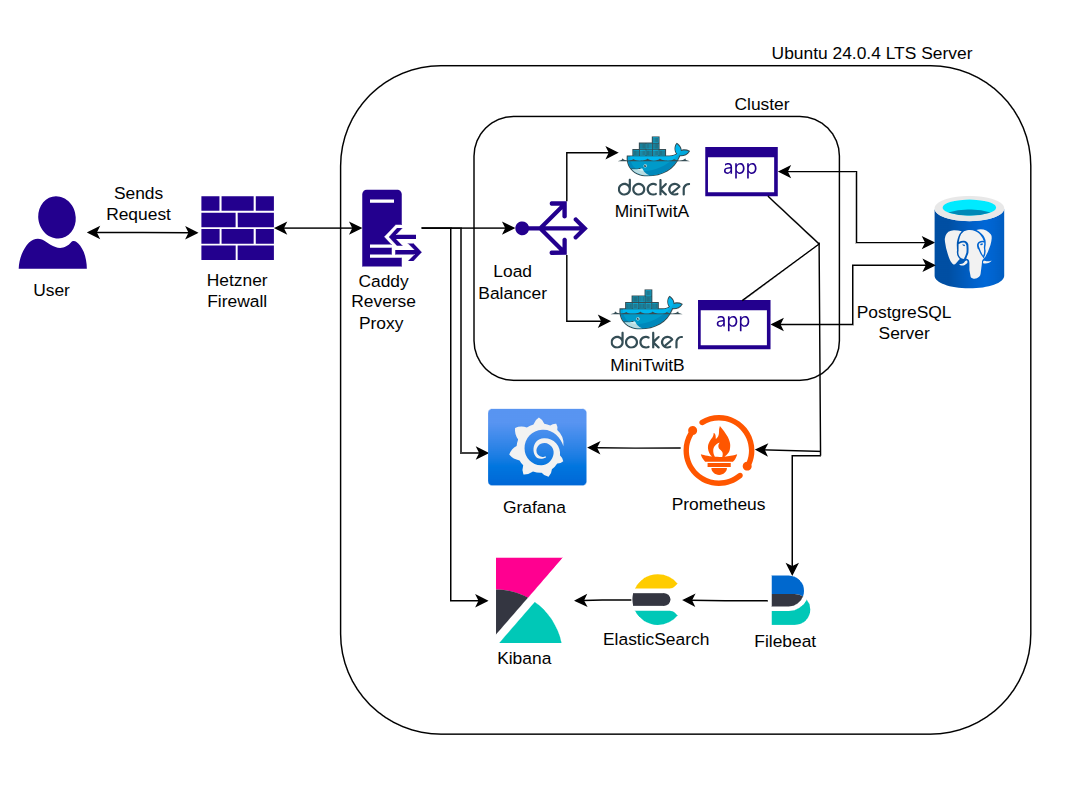
\includegraphics[width=0.8\linewidth]{report/images/Minitwit_diagram.png}
    \caption{Minitwit System Overview}
    \label{fig:Minitwit System Overview}
\end{figure}